\documentclass[11pt]{article}
\usepackage[margin=21mm]{geometry}
\usepackage{lmodern}
\usepackage[T1]{fontenc}
\usepackage{amsmath}
\usepackage[strings]{underscore}   % literal _ in text/texttt (K_d etc. stay math)
\usepackage{microtype}
\usepackage{xcolor}
\usepackage{booktabs}
\usepackage{enumitem}
\usepackage{titlesec}
\usepackage{tikz}
\usetikzlibrary{positioning,arrows.meta,calc,fit,backgrounds}
\usepackage[colorlinks=true,linkcolor=tealc,urlcolor=tealc,citecolor=tealc]{hyperref}

% ---- project palette --------------------------------------------------------
\definecolor{coral}{HTML}{B85B3A}
\definecolor{tealc}{HTML}{2A6478}
\definecolor{forest}{HTML}{3D6E4A}
\definecolor{plum}{HTML}{5A4A6A}
\definecolor{char}{HTML}{2A2520}
\definecolor{dimc}{HTML}{6E6862}
\definecolor{gridc}{HTML}{E8E5E0}
\definecolor{coralL}{HTML}{F4D6CB}
\definecolor{tealL}{HTML}{D6E3E8}
\definecolor{forestL}{HTML}{D8E5DC}
\definecolor{plumL}{HTML}{E3DEEA}
\definecolor{sand}{HTML}{F5F1EA}

\setlist[itemize]{leftmargin=1.3em, itemsep=1.5pt, topsep=2pt}
\titlespacing*{\section}{0pt}{12pt}{5pt}
\titlespacing*{\subsection}{0pt}{9pt}{3pt}
\titleformat{\section}{\Large\bfseries\color{char}}{\thesection}{0.6em}{}
\titleformat{\subsection}{\large\bfseries\color{tealc}}{}{0em}{}
\newcommand{\code}[1]{\texttt{\small #1}}
\newcommand{\fn}[1]{\texttt{\small\color{coral}#1}}

% ---- shared TikZ styles -----------------------------------------------------
\tikzset{
  arr/.style={-{Stealth[length=5pt,width=5pt]}, line width=0.9pt, color=char, rounded corners=3pt},
  eng/.style={draw=tealc, fill=tealL, rounded corners=2.5pt, font=\ttfamily\small,
              inner sep=5pt, minimum height=8mm, align=center},
  fnd/.style={draw=dimc, fill=sand, rounded corners=2.5pt, font=\ttfamily\small,
              inner sep=5pt, minimum height=8mm, align=center},
  dat/.style={draw=forest, fill=forestL, rounded corners=2.5pt, font=\ttfamily\small,
              inner sep=5pt, minimum height=8mm, align=center},
  lay/.style={draw=char, rounded corners=3pt, align=center, inner sep=6pt,
              font=\small, minimum width=8.4cm},
  hot/.style={draw=coral, fill=coralL, rounded corners=2.5pt, font=\ttfamily\small,
              inner sep=5pt, minimum height=8mm, align=center},
}

\begin{document}

% =============================================================================
\begin{center}
  {\LARGE\bfseries\color{char} Lunar-HFE — Code Manual}\\[3pt]
  {\color{dimc} How the code works, what each \texttt{.py} file does,
   and how the files connect.}
\end{center}
\vspace{2pt}

\noindent
This is the \textbf{file-level} companion to \code{CODE_TOUR.md (in documents/dev/)} (the
folder-level tour) and the \emph{guidebook} (the physics). It names every
module, says what it contributes, and draws the import graph so you can trace
one number from raw Apollo data to the paper. The project retrieves the deep
regolith thermal conductivity $K_d$ at the Apollo~15 and~17 heat-flow
boreholes by fitting a 1-D thermal model to the measured subsurface
temperatures.

% =============================================================================
\section{The four layers, one rule}

The code is organized as four layers. \textbf{The one rule:} dependencies only
ever point \emph{downward} — the engine never imports the pipeline; the
pipeline never imports a figure script. That is what keeps the physics testable
in isolation and the results reproducible.

\begin{center}
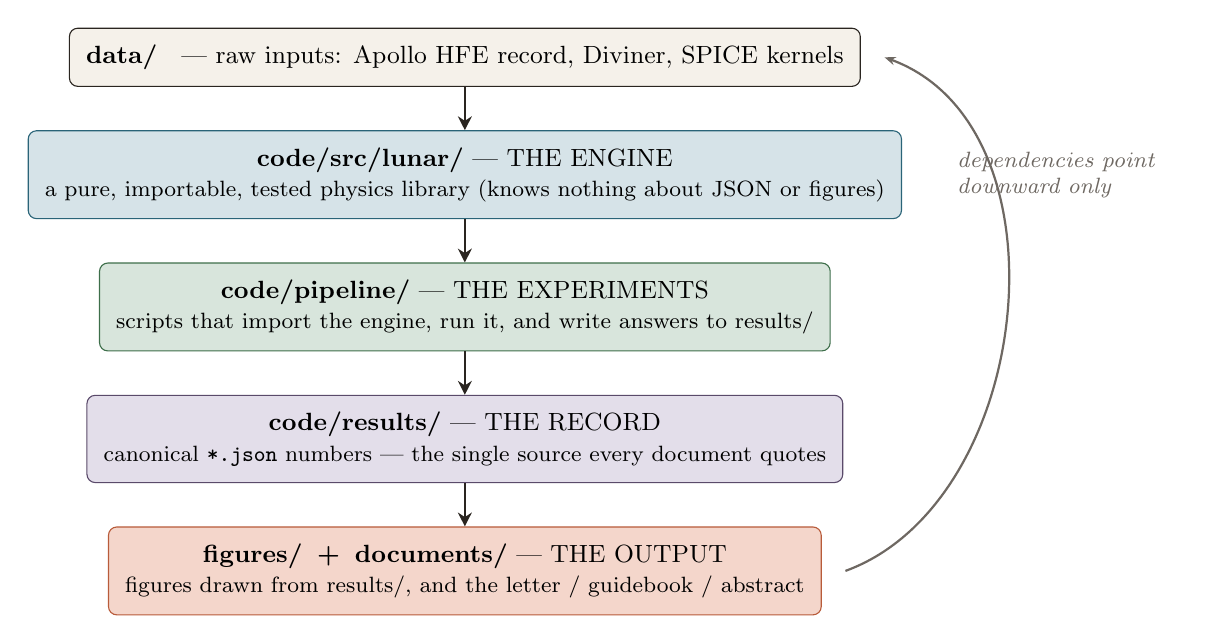
\begin{tikzpicture}[node distance=5.5mm]
  \node[lay, fill=sand]                     (data) {\textbf{data/} \; — raw inputs: Apollo HFE record, Diviner, SPICE kernels};
  \node[lay, fill=tealL,  draw=tealc, below=of data] (eng)  {\textbf{code/src/lunar/} — THE ENGINE\\ \footnotesize a pure, importable, tested physics library (knows nothing about JSON or figures)};
  \node[lay, fill=forestL,draw=forest, below=of eng]  (pipe) {\textbf{code/pipeline/} — THE EXPERIMENTS\\ \footnotesize scripts that import the engine, run it, and write answers to results/};
  \node[lay, fill=plumL,  draw=plum, below=of pipe]  (res)  {\textbf{code/results/} — THE RECORD\\ \footnotesize canonical \texttt{*.json} numbers — the single source every document quotes};
  \node[lay, fill=coralL, draw=coral, below=of res]  (out)  {\textbf{figures/ \,+\, documents/} — THE OUTPUT\\ \footnotesize figures drawn from results/, and the letter / guidebook / abstract};
  \foreach \a/\b in {data/eng, eng/pipe, pipe/res, res/out} \draw[arr] (\a) -- (\b);
  \node[right=6mm of eng, text width=2.9cm, font=\footnotesize\itshape, text=dimc]
        {dependencies point downward only};
  \draw[-{Stealth[length=4pt]}, dimc, thick]
        ([xshift=3mm]out.east) to[out=20,in=-20] ([xshift=3mm]data.east);
\end{tikzpicture}
\end{center}

% =============================================================================
\section{How the engine files connect}

Every module in \code{code/src/lunar/} and which internal modules it imports
(read from the source, not guessed). \textbf{\code{constants} is the floor};
\code{config}, \code{grid}, \code{properties} build on it; \code{solver} sits
on those; \code{equilibrium} sits on the solver. No import cycles.

\begin{center}
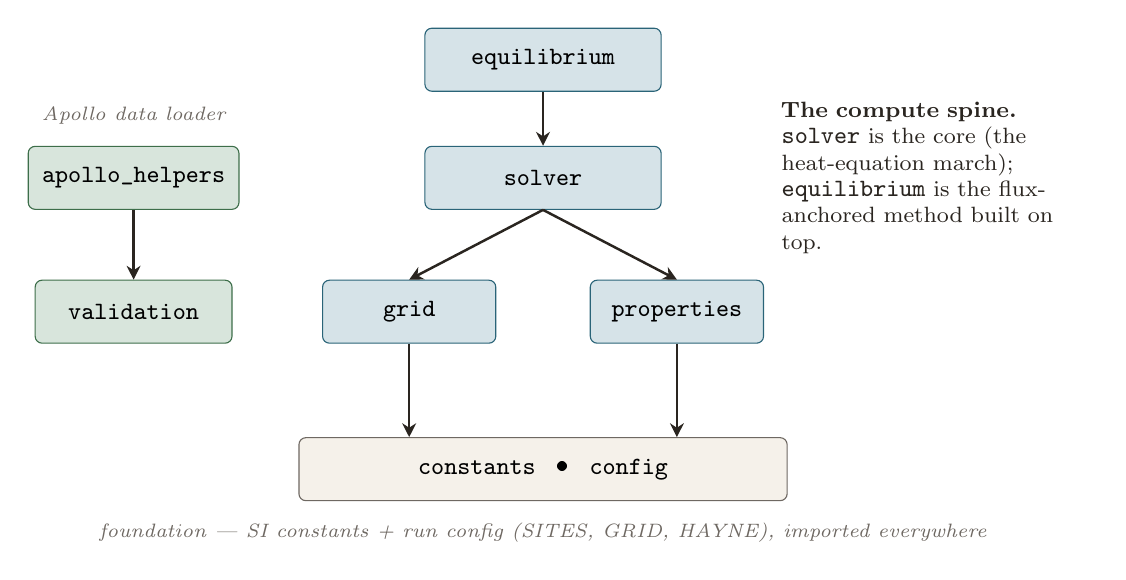
\begin{tikzpicture}
  % single foundation box
  \node[fnd, minimum width=6.2cm] (found) at (0,0) {constants \;\textbullet\; config};
  \node[font=\scriptsize\itshape, text=dimc, below=1.5mm of found]
        {foundation — SI constants + run config (SITES, GRID, HAYNE), imported everywhere};

  % spine: grid / properties -> solver -> equilibrium
  \node[eng, minimum width=2.2cm] (grid)  at (-1.7,2.0) {grid};
  \node[eng, minimum width=2.2cm] (props) at ( 1.7,2.0) {properties};
  \node[eng, minimum width=3.0cm] (solver) at (0,3.7) {solver};
  \node[eng, minimum width=3.0cm] (equil)  at (0,5.2) {equilibrium};

  \draw[arr] (grid.south)  -- (grid.south  |- found.north);
  \draw[arr] (props.south) -- (props.south |- found.north);
  \draw[arr] (solver.south) -- (grid.north);
  \draw[arr] (solver.south) -- (props.north);
  \draw[arr] (equil.south) -- (solver.north);

  % annotation (right, clear space)
  \node[right=14mm of solver, text width=3.9cm, font=\footnotesize, text=char]
    {\textbf{The compute spine.} \code{solver} is the core (the heat-equation
     march); \code{equilibrium} is the flux-anchored method built on top.};

  % data-loader chain (far left, own column)
  \node[dat, minimum width=2.5cm] (apollo) at (-5.2,3.7) {apollo\_helpers};
  \node[dat, minimum width=2.5cm] (valid)  at (-5.2,2.0) {validation};
  \draw[arr] (apollo.south) -- (valid.north);
  \node[font=\scriptsize\itshape, text=dimc, above=1.5mm of apollo, align=center]
        {Apollo data loader};
\end{tikzpicture}\\[2pt]
{\footnotesize\itshape\color{dimc} Leaf helpers (no internal deps), used
across the pipeline: ephem (SPICE) \textbullet\ diviner \textbullet\
plotting/style \textbullet\ \_bootstrap.}
\end{center}

% =============================================================================
\section{The engine, file by file \; (\texttt{code/src/lunar/})}

\begin{description}[leftmargin=0pt, labelsep=0.4em, style=nextline, itemsep=3pt]
\item[\fn{constants.py} — the physical floor]
  All SI physical constants and default regolith parameters, each with a source
  citation ($\sigma$, $S_0$, $K_s$, $H$, $\chi$, $T_\text{ref}$, the Hayne
  $c_p$ polynomial, Martínez coefficients). \emph{No internal deps.} Never add a
  number here without a citation.
\item[\fn{config.py} — single source of truth for a run]
  The per-site table \code{SITES} (lat/lon, albedo, \code{Q_BASAL}), the grid
  spec \code{GRID} (\code{z_max=5.0}, \code{dz0=0.002}, \code{growth=0.08}), the
  \code{HAYNE} bundle, \code{DT_STEP}, and \code{EQ_Z_ANCHOR=0.55},
  \code{EQ_N_INNER=96}. \textbf{Uses} constants. Import it; never redefine.
\item[\fn{grid.py} — the geometric depth grid]
  \fn{make_geometric_grid()} builds the non-uniform column (2\,mm surface cells
  coarsening to 5\,m) as a frozen \code{DepthGrid}. Uniform spacing is
  forbidden. \textbf{Uses} constants.
\item[\fn{properties.py} — the material models $K(T,z)$, $\rho(z)$, $c_p(T)$]
  \fn{conductivity_hayne} (baseline, contact\,$\times$\,radiative — the letter's
  model), \fn{conductivity_martinez} (the $K(T,\rho)$ alternative),
  \fn{density_hayne}, \fn{specific_heat}, all reachable via
  \fn{get_conductivity_model}. \textbf{Uses} constants.
\item[\fn{solver.py} — THE CORE: the 1-D heat-equation solver]
  Marches $\rho c_p\,\partial_t T = \partial_z(K\partial_z T)$ in time — where
  essentially all compute cost lives. Inner$\to$outer: \fn{_thomas} (tridiagonal
  solve, the innermost hot op), \fn{_face_harmonic_mean},
  \fn{_solve_surface_newton}, \fn{_step} (one Crank–Nicolson hour),
  \fn{_march_radiative_hayne} (the \code{@njit} lunation march \emph{the C++
  port mirrors}), \fn{solve_pixel} (public forward-solve entry).
  \textbf{Uses} config, constants, grid, properties.
\item[\fn{equilibrium.py} — THE METHOD: flux-anchored steady state]
  The ``slope method'' — reaches the periodic steady state $\sim$20$\times$
  faster than brute force. \fn{solve_periodic_equilibrium} (public entry),
  \fn{_reconstruct_subskin} (Step~B: walk the deep profile down the closure ODE
  $d\langle T\rangle/dz=(Q_b-u_\text{rect})/K$), \fn{_rectified_flux},
  \fn{_mean_flux_closure} (convergence test), \fn{profile_at_time}.
  \textbf{Uses} solver, config, constants, grid.
\item[\fn{apollo_helpers.py} — raw record $\to$ fit targets]
  \fn{extract_sensor_stability(mission, min_depth_cm)} returns each sensor's
  depth, equilibrium temperature $T_\text{eq}$, scatter, and the
  \code{deep_mask} (sensors past the 80\,cm borestem zone). \textbf{Uses}
  validation.
\item[\fn{validation.py} — the Apollo HFE data loader]
  Low-level reader for the bundled Apollo 15/17 depth tables (Nagihara 2018).
  \emph{Leaf.}
\item[\fn{ephem.py} \;/\; \fn{diviner.py} — external data access]
  \code{ephem}: SPICE solar geometry (for ephemeris-driven pixel solves).
  \code{diviner}: Diviner GCP surface temperatures (surface-closure test).
  \emph{Leaves.}
\item[\fn{plotting/style.py} — the figure identity]
  JGR:Planets rcParams, palette (\code{C_A15}, \code{C_A17}, \code{WARM_DIVERGE}
  \ldots), and helpers (\fn{fmt_axis}, \fn{legend_below},
  \fn{assert_no_overlap}). Every figure script imports it.
\item[\fn{_bootstrap.py} — notebook convenience]
  \fn{find_repo_root()} so a notebook runs from a clean checkout. \emph{Leaf.}
\end{description}

% =============================================================================
\section{The pipeline \; (\texttt{code/pipeline/})}

Scripts that \emph{use} the engine — they orchestrate physics and write JSON;
they never define physics.

\begin{itemize}
\item \fn{compute/retrieve_kd.py} — \textbf{the orchestrator (start here).}
  Reads the HFE record, sweeps $K_d$, fits the best value per site, bootstraps
  the CI, writes \code{results/kd_retrieval_results.json}. Key functions:
  \fn{run_with} (one model evaluation at a given $K_d$), \fn{run_kd_sweep_extended}
  (the RMSE sweep), \fn{kd_star_from_residuals} (parabolic vertex $\to K_d^{*}$),
  \fn{bootstrap_kd_with_depth_uncertainty}, \fn{main}. Uses nearly the whole engine.
\item \textbf{compute/ — auxiliary scripts} (each writes one \code{results/*.json},
  same shape: import engine $\to$ compute $\to$ dump JSON):
  \emph{sensitivity} (\code{compute_borestem_sensitivity},
  \code{compute_common_epoch}, \code{compute_stability_threshold_sensitivity},
  \code{compute_surface_bias_test}, \code{compute_fixed_input_sensitivities},
  \code{compute_uniform_kd_sensitivity});
  \emph{model comparison} (\code{compute_headline_rmse},
  \code{compute_model_selection}, \code{compute_error_budget});
  \emph{$Q_b$ / Bayesian} (\code{compute_qb_degeneracy}, \code{bayesian_crosscheck},
  \code{qb_prior_width_scan});
  \emph{numerics} (\code{convergence_scan}, \code{dt_ladder},
  \code{check_discretization});
  \emph{surface closure} (\code{compute_diviner_closure});
  \emph{speed} (\code{benchmark_speedup}, \code{benchmark_cpp}).
\item \textbf{figures/} — $\sim$38 \code{make_*.py}. One pattern: import
  \code{plotting.style}, read a \code{results/*.json}, draw, save a PDF into
  \code{figures/}. They read numbers; they never recompute physics.
\item \textbf{top-level:} \fn{make_all_figures.py} (runs every generator),
  \fn{fetch_diviner.py} (one-time data download),
  \fn{extract_lola_relief.py} (context-map crops), \fn{run_all_timed.py}.
\end{itemize}

% =============================================================================
\section{The one journey: a $K_d$ number, end to end}

Follow this once and the rest is detail. Everything above the coral box runs
once per $K_d$; the coral march runs for every hour of every lunation — which is
why the solver is the entire cost.

\begin{center}
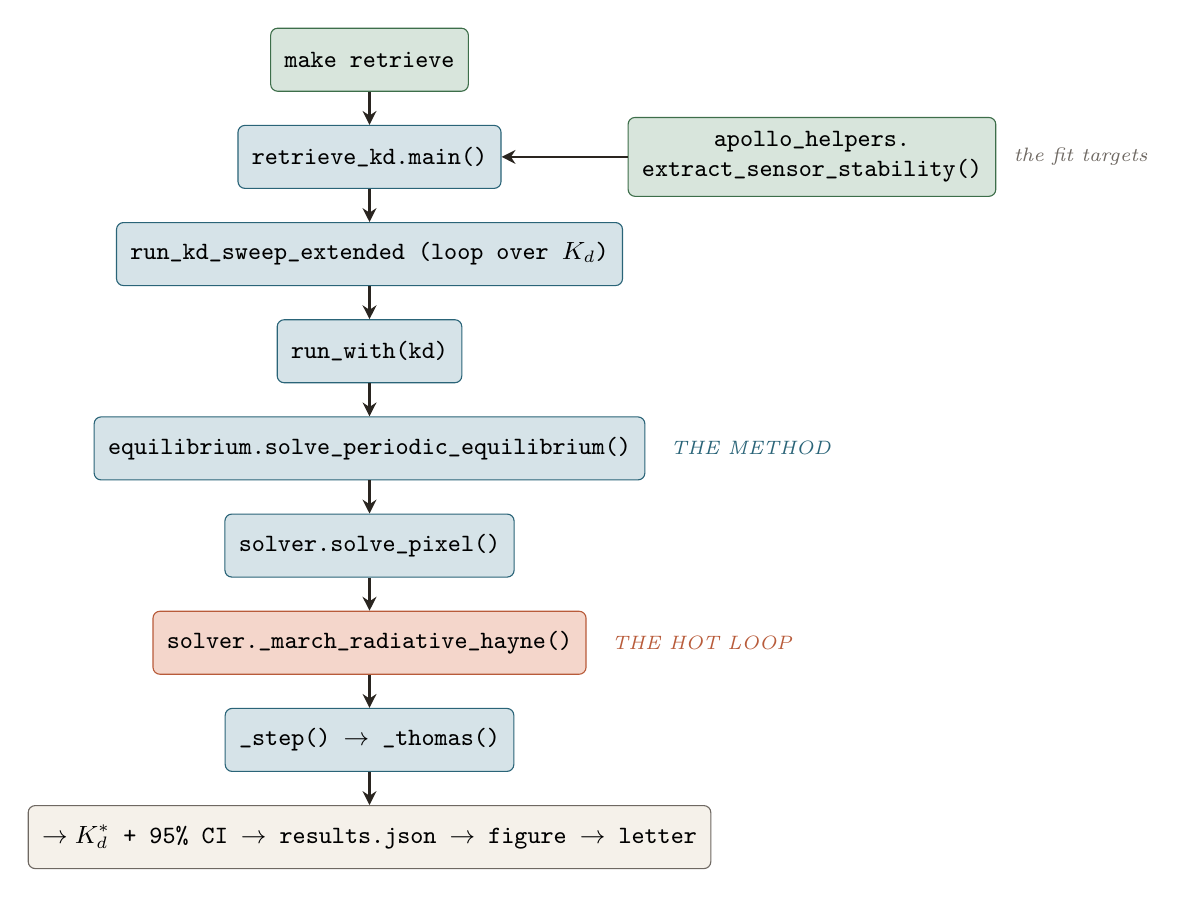
\begin{tikzpicture}[node distance=4.2mm, every node/.style={font=\ttfamily\small}]
  \node[dat]                          (mk)   {make retrieve};
  \node[eng, below=of mk]             (main) {retrieve_kd.main()};
  \node[eng, below=of main]           (sweep){run_kd_sweep_extended  (loop over $K_d$)};
  \node[eng, below=of sweep]          (rw)   {run_with(kd)};
  \node[eng, below=of rw, fill=tealL, draw=tealc] (eq) {equilibrium.solve_periodic_equilibrium()};
  \node[eng, below=of eq]             (sp)   {solver.solve_pixel()};
  \node[hot, below=of sp]             (march){solver.\_march_radiative_hayne()};
  \node[eng, below=of march]          (step) {\_step()  $\to$  \_thomas()};
  \foreach \a/\b in {mk/main, main/sweep, sweep/rw, rw/eq, eq/sp, sp/march, march/step}
     \draw[arr] (\a) -- (\b);
  % side targets branch
  \node[dat, right=16mm of main, align=center] (ex) {apollo\_helpers.\\extract_sensor_stability()};
  \draw[arr] (ex.west) -- (main.east);
  \node[font=\scriptsize\itshape\rmfamily, text=dimc, right=1mm of ex] {the fit targets};
  % labels
  \node[font=\scriptsize\itshape\rmfamily, text=tealc, right=2mm of eq]   {THE METHOD};
  \node[font=\scriptsize\itshape\rmfamily, text=coral, right=2mm of march]{THE HOT LOOP};
  % tail
  \node[fnd, below=of step, align=center] (out)
        {$\to K_d^{*}$ + 95\% CI $\to$ results.json $\to$ figure $\to$ letter};
  \draw[arr] (step) -- (out);
\end{tikzpicture}
\end{center}

% =============================================================================
\section{The C++ port \; (\texttt{code/cpp/solver.cpp})}

A faithful, dependency-free $\sim$300-line C++ port of \emph{only} the solver
hot loop (\fn{_march_radiative_hayne}) — same equations, same order.
\fn{benchmark_cpp.py} feeds it a binary blob and reads the result; grid
construction and forcing stay in Python (no duplicated definitions). Notebook
\code{06_performance.ipynb} compiles it and runs all three engines on identical
inputs.

\begin{center}\small
\begin{tabular}{@{}lrl@{}}
\toprule
engine & ms\,/\,lunation & speed \\
\midrule
generic Python      & $\sim$550 & 1$\times$ \\
\textbf{Numba (production)} & $\sim$4.8 & \textbf{$\sim$115$\times$} \\
C++ port            & $\sim$3.2 & $\sim$170$\times$ ~(only \textbf{1.5$\times$} over Numba)\\
\bottomrule
\end{tabular}
\end{center}

\noindent
\textbf{Important:} the production pipeline runs on \textbf{Numba, not C++}. The
$\sim$100$\times$ win is Numba over interpreted Python; the C++ adds only
$\sim$1.5$\times$. Its value is (a) a language-independent correctness witness
(the three engines agree to $\sim$10$^{-12}$\,K) and (b) a path to a
dependency-free, parallelizable kernel for a large job such as a full-Moon map.

% =============================================================================
\section{Running it}

\begin{center}\small
\begin{tabular}{@{}ll@{}}
\toprule
command & what it does \\
\midrule
\code{make retrieve} & core retrieval + bootstrap $\to$ \code{kd_retrieval_results.json} \\
\code{make aux}      & sensitivity sweeps, model selection, error budget, MCMC \\
\code{make figures}  & regenerate every figure into \code{figures/} \\
\code{make paper}    & compile the letter + guidebook \\
\code{make test}     & unit tests (\code{pytest}, 49 tests) \\
\code{make all}      & the whole chain: retrieve $\to$ aux $\to$ figures $\to$ paper \\
\bottomrule
\end{tabular}
\end{center}

\noindent
\textbf{Notebooks} (\code{code/notebooks/}, in order):
\code{00_setup} $\to$ \code{01_methods} $\to$ \code{02_retrieval} $\to$
\code{03_results} $\to$ \code{04_discussion} $\to$ \code{05_method} (the
flux-anchored method) $\to$ \code{06_performance} (Python vs Numba vs C++, and
scaling to a map).

\end{document}
